\subsection{Evaluasi Pengujian \textit{Smart Contract}}

Hasil eksekusi pengujian menunjukkan seluruh skenario pengujian berhasil dijalankan.
Total terdapat sembilan \textit{test} yang dijalankan, dengan hasil sembilan \textit{test} berhasil dan tidak ada \textit{test} yang gagal.
Hasil pengujian dapat dilihat pada Tabel~\ref{tab:expected-output-smart-contract} dan pada Gambar~\ref{fig:smart-contract-test-result}.

\begin{figure}[htbp]
	\centering
	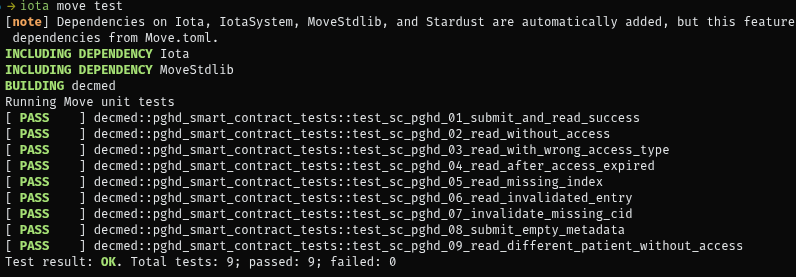
\includegraphics[width=\textwidth]{resources/chapter-4/pengujian_sc.png}
	\caption{Hasil Pengujian \textit{Smart Contract}}\label{fig:smart-contract-test-result}
\end{figure}


\begin{styledxltabular}{|>{\raggedright\arraybackslash}p{0.10\textwidth}|>{\raggedright\arraybackslash}p{0.22\textwidth}|>{\raggedright\arraybackslash}X|>{\raggedright\arraybackslash}p{0.26\textwidth}|>{\raggedright\arraybackslash}p{0.10\textwidth}|}
    \hiderowcolors
    \caption{Ekspektasi Balikan Pengujian \textit{Smart Contract} PGHD}\label{tab:expected-output-smart-contract} \\
    \hline
    \rowcolor{headerBg}
    \textbf{Kode} & \textbf{Skenario} & \textbf{Ekspektasi Hasil} & \textbf{Ekspektasi Balikan} & \textbf{Hasil} \\
    \hline
    \showrowcolors
    \endfirsthead
    \hline
    \rowcolor{headerBg}
    \textbf{Kode} & \textbf{Skenario} & \textbf{Ekspektasi Hasil} & \textbf{Ekspektasi Balikan} & \textbf{Hasil} \\
    \hline
    \endhead
    \hline
    \endfoot
    \hline
    \endlastfoot
    T-SC-01 & \textit{Submit} dan baca PGHD dengan akses valid. & Daftar PGHD berisi satu \textit{metadata} dan detail \textit{index} 0 dapat dibaca. & \texttt{PASS} & Sukses \\
    \hline
    T-SC-02 & Baca PGHD tanpa akses. & Akses ditolak karena \textit{access token} tidak ditemukan. & \texttt{EAccess\-NotFound} & Sukses \\
    \hline
    T-SC-03 & Baca PGHD memakai akses \textit{medical record}. & Akses ditolak karena tipe akses tidak sesuai dengan PGHD\@. & \texttt{EInvalid\-Access\-Type} & Sukses \\
    \hline
    T-SC-04 & Baca PGHD setelah akses \textit{expired}. & Akses ditolak karena melewati durasi akses yang diizinkan. & \texttt{EAccess\-Expired} & Sukses \\
    \hline
    T-SC-05 & Buka \textit{index} PGHD yang tidak ada. & Detail PGHD tidak dikembalikan karena \textit{index} tidak ditemukan. & \texttt{EPGHD\-Record\-NotFound} & Sukses \\
    \hline
    T-SC-06 & Buka entri PGHD yang \textit{invalid}. & Entri ditolak karena data sudah ditandai tidak valid. & \texttt{EPGHD\-Record\-Invalid} & Sukses \\
    \hline
    T-SC-07 & \textit{Invalidate} CID PGHD yang tidak ada. & Operasi invalidasi ditolak karena CID tidak ditemukan. & \texttt{EPGHD\-Record\-NotFound} & Sukses \\
    \hline
    T-SC-08 & \textit{Submit} \textit{metadata} PGHD kosong. & \textit{Metadata} tidak disimpan karena tidak memenuhi validasi minimum. & \texttt{EInvalid\-Pghd\-Metadata} & Sukses \\
    \hline
    T-SC-09 & Baca PGHD pasien berbeda. & Akses ditolak karena \textit{grant} akses tidak berlaku untuk pasien tersebut. & \texttt{EAccess\-NotFound} & Sukses \\
    \hline
\end{styledxltabular}
